\chapter{Integration of the proposed model within the ILUTE framework }

This chapter outlines the ILUTE labour market module changes necessary to integrate the proposed salary model. Moreover, it evaluates the proposed model relative to the current implementation using several performance criteria. Although this integration is out of the scope of this thesis, it provides an informed opinion about its potential performance within that framework. 

\section{Integration of the proposed salary model with the existing implementation }

Given the difference between the outputs in the existent wage model and the proposed salary model, it is necessary to modify the salary representation within the ILUTE framework. According to \citet{Harmon2013}, salaries are represented in ILUTE as an attribute within the Person class. This attribute corresponds to the numerical value \textit{Wage} that stores the hourly wage of each agent. However, in the proposed salary model, the prediction result is a list of values representing the annual salary distribution for that person at that time step. Therefore, the \textit{Wage} attribute in the Person class needs to be replaced by two attributes: 

\begin{itemize}
    \item \textit{\textbf{Current\_salary}} stores the salary value resulting from the job matching process known as \textit{FinalOffer} \citep{Harmon2013}. This value plays the same role as the \textit{Wage} attribute within the ABM but differs in its units.
    \item \textit{\textbf{Reference\_salary}} stores the list of values from the proposed salary model and represents the market salary distribution for an individual with such characteristics at the current time step. The size of this list corresponds to the number of samples defined in the prediction step. As shown in \Cref{fig:class_person}, more samples will improve the precision but increase the memory requirements for each run and the running time for salary calculations (e.g. calculate the expected salary value for each person or compare salary distribution between individuals). Then, the right balance between sample size and precision should be decided according to the available computational resources and the running times. 
\end{itemize}

Then, the Job-matching procedure remains the same, except that the \textit{MinimumWageAccepted}, Worker's utility $\Delta V(best)$, and all premium and discount percentages\footnote{\textit{MarketAdjustmentFactor}, the premium for being employed, the discount for entering the Workforce, and the premium or discount for each matching attempt for both firm and worker: \textit{JobApplicationAttempts} and \textit{FailedRecruitingAttempts}} are calculated with respect to the expected value of the \textit{Reference\_salary}.

\begin{figure}[h]
    \centering
    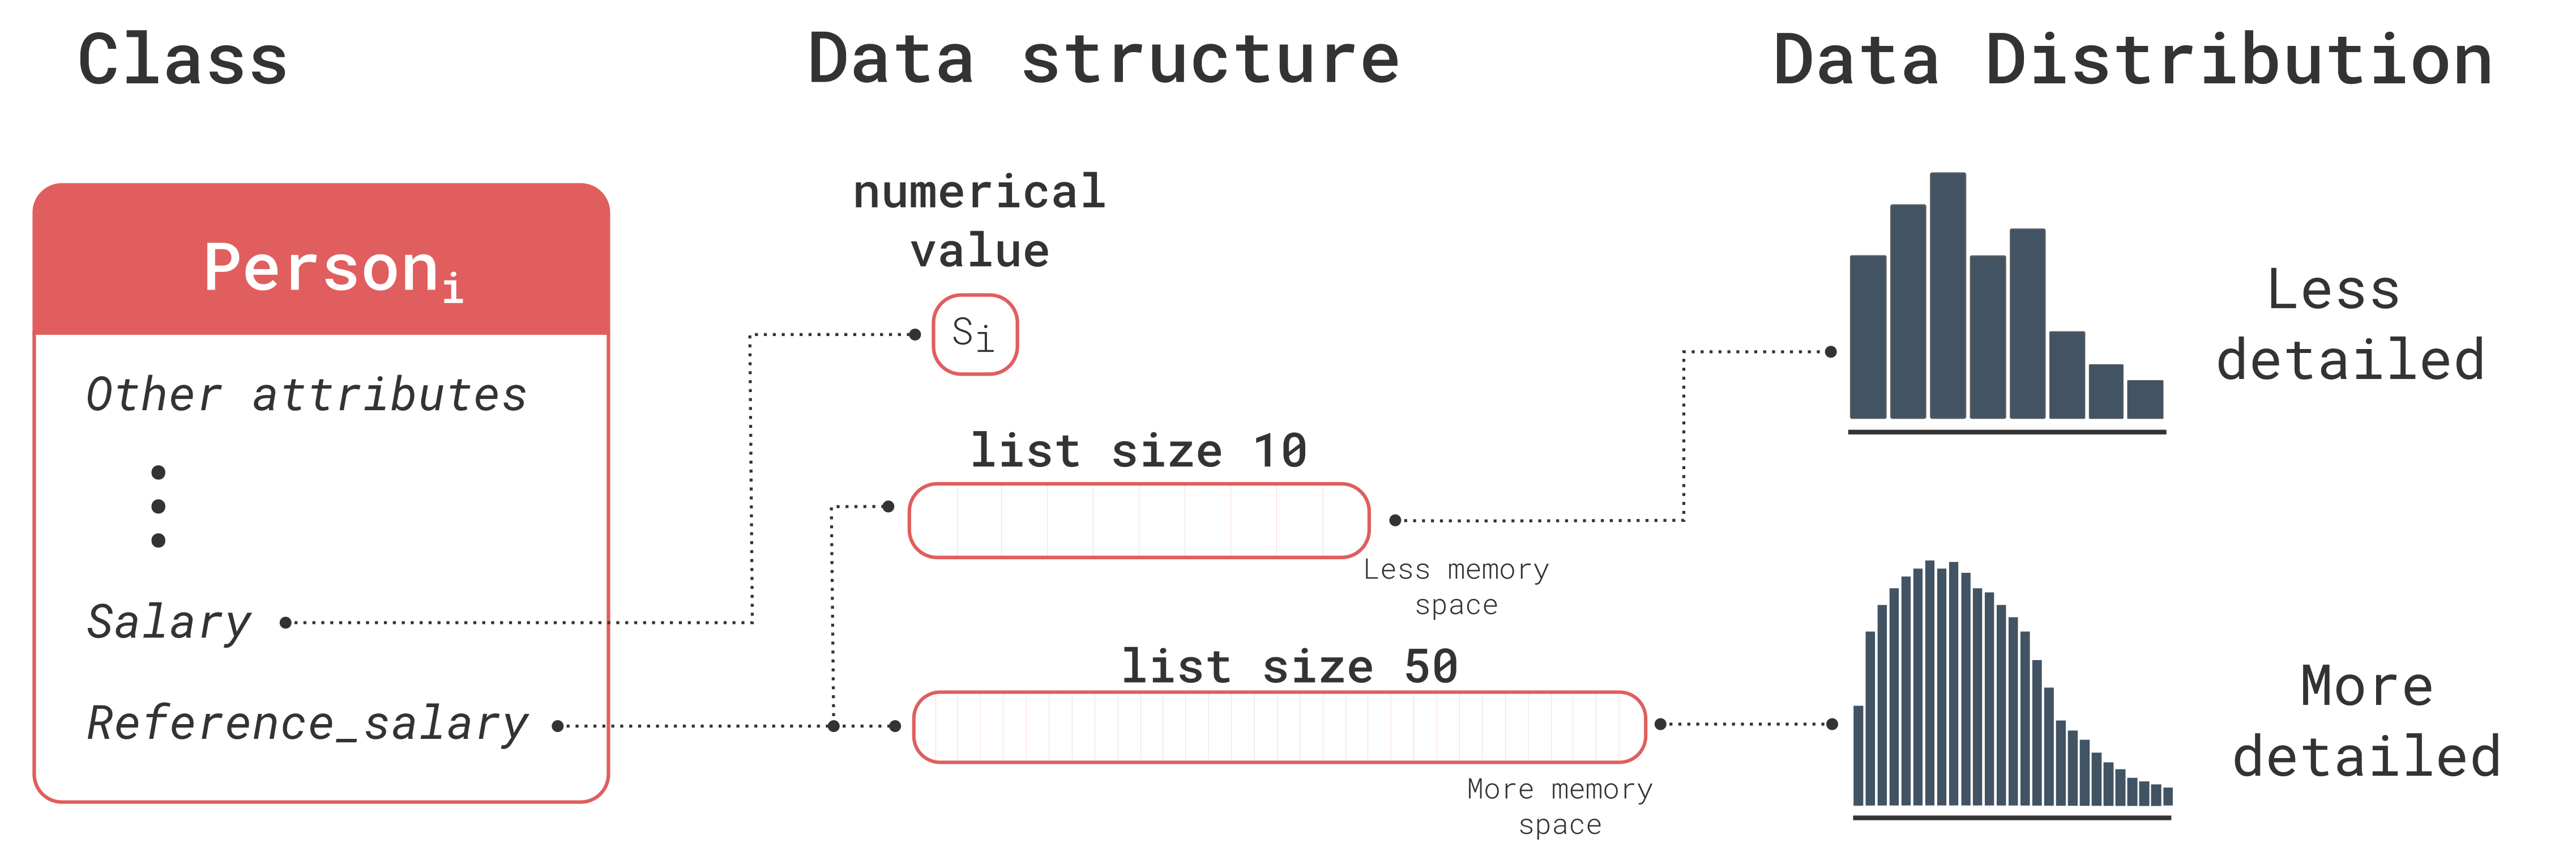
\includegraphics[width=0.8\textwidth]{images/ch6_class_person/class_person.png}
    \caption{Proposed salary representation in ILUTE.}
    \setlength{\abovecaptionskip}{-15pt}
    \label{fig:class_person}
\end{figure}

\section{Model comparison: proposed vs existent salary model}

As the units of the target variable in the existing and proposed model differ, a direct comparison between performance metrics might not be the best approach to compare them. Hence, the following list compares both models based on different criteria such as performance, computation efficiency, and suitability within the ILUTE framework.

\begin{itemize}
    \item \textbf{Model capability}: In the original implementation, \citet{Hain2010} defined a series of interaction terms to improve the model's performance. These interaction terms capture the complex relationships and dependencies between the variables, but this process is performed manually. In the proposed model, the hierarchical structure captures these relationships and dependencies without using any manual process. Therefore, the proposed model is a better approach for representing these dependencies between variables without risking the introduction of some bias in the model. 
    \item \textbf{Model Interpretability}: Although introducing predictor variables could increase model performance, it directly reduces the model's interpretability. This would not be an issue in some settings where prediction accuracy is the aim. However, interpretability becomes very important when the model objective is to support public policy decisions, such as in ILUTE. Therefore, the proposed model contains ten variables with no explicit interaction terms, which allows a more straightforward interpretation of the model results and parameter meaning.
    \item \textbf{Model complexity}: There is a direct relationship between the number of predictors (variables and interaction terms) and the model complexity. The higher the model complexity, the higher the risk of overfitting the data, which decreases the model's ability to generalize on new data and reduces the model's robustness to structural changes in the future labour market. The shrinkage effect observed in \Cref{section:structure_selection} and using a holdout dataset to measure the real performance \Cref{section:model_validation}, reduces the risk of overfitting and improves the model's generalization capability.
    \item \textbf{Model purpose and usability}: The labour market usually involves random variations and uncertainty in its processes and outputs. For instance, two individuals with the same attributes can have salary differences explained by random factors such as belonging to a company that pays better or having better negotiation skills. Although some systematic components explain most salary distribution, some can only be explained by introducing randomness in the modelling process. This randomness makes salary prediction a stochastic process in nature. However, the original implementation of the wage model produces a deterministic output, which means that a set of initial conditions will always produce the same outputs. Given the simulation nature of the ILUTE framework, the proposed model seems to be a better approach to introduce this random component in the prediction by producing distributions instead of point estimates. In particular, these distributions might improve the job-matching algorithm and the overall ABM process proposed by \citet{Harmon2013}. On the other hand, as the ILUTE framework is supposed to be used in a public policy evaluation setting, a what-if evaluation could benefit more from a stochastic perspective than a deterministic one by accounting for the uncertainty in the estimation of the results both at the aggregate or disaggregated level.
    \item \textbf{Model robustness and flexibility}: In the long term, the labour market evolves by introducing or eliminating some industries and occupations, adjusting the market to political and cultural changes, and reflecting technological changes in the salaries received by workers in a specific sector, among others. The hierarchical structure of the proposed model eases the introduction of these changes, as new industries and occupations generally share some characteristics with the existing industries. Hence, the information transfer between different levels in the proposed model produces better prediction under these changing scenarios. Even if this first guess is not accurate, the online learning structure in the Bayesian approach helps to update these estimates in the light of new data. Conversely, the original model must be entirely estimated when new data is available or when there are significant changes in the labour market structure. This estimation could require a significant effort and produce contradictory results between each estimation because there is no way to use the previous parameters in the new estimation process.
    \item \textbf{Model inference efficiency}: The advantages of the proposed model discussed in the last bullets come with a cost. The complexity of the estimation process increases considerably in the proposed model because new processes, such as the prior definition and the sampling process, are additional steps compared with the simplicity of the ordinary least squares (OLS) of the existent model. Given the probabilistic nature of the sampling process, this is a slow and computationally inefficient process because a percentage of the samples are discarded, which means that a portion of the allocated computational power is wasted. Despite recent improvements in efficient alternatives to MCMC, this process is still slow compared to the original approach (OLS). A way to mitigate this issue is to define the priors that represent the observed phenomena carefully. This helps the model converge more efficiently and reduces the number of discarded samples. 
    \item \textbf{Model memory usage}: Although the proposed model provides more information than the original approach, this advantage could become a disadvantage because this information needs to be stored and handled adequately. While the memory constraint is an issue that is becoming less important as powerful hardware is getting cheaper (Moore's Law), it is still relevant when dealing with a multi-agent simulation environment. In this case, an adequate model implementation27 and a proper sample size definition can help reduce memory usage while producing helpful information. 

    \item \textbf{Model scalability}: Although this topic applies to both approaches, it is known that MCMC sampling scales poorly as more data is added to the model. To mitigate this effect, it is crucial to define the process of updating the model parameters using approaches like the one discussed in Section 5.6. This is an advantage of the proposed model compared to the original approach because the existing model needs to be estimated from scratch in the light of new data. However, the difference in the computational cost of both approaches is better for the original model. 
    
    \item \textbf{Temporal scale representation}: The existing model generates estimates at the hourly level, and the proposed model predicts salaries at the annual scale. While the proposed model can produce better estimates of the individual annual income, the hourly approach of the existent model provides more flexibility to model different temporal scales as hourly salary can be aggregated into several representations such as daily, monthly or annually. However, as pointed out in Harmon's work, some assumptions about the number of work hours per week can induce estimation errors, affecting the original model's reliability and performance. 
\end{itemize}






 




